\section{Анализ технического задания на курсовое проектирование}
\label{sec:analysis}

\subsection{Анализ предметной области}

На сегодняшний день не существует аспектов работы вокзалов, которые бы не были связаны с применением информационных технологий. Благодаря современным информационным системам деятельность вокзалов, как узловых точек транспортной инфраструктуры, осуществляется эффективно и с высокой степенью автоматизации. Эти системы позволяют оптимизировать различные процессы, улучшить качество обслуживания пассажиров и повысить безопасность на объектах.

Информационные технологии и компьютеризация вокзалов позволяют усовершенствовать и ускорить процессы управления пассажирскими потоками, обработки данных, организации транспортных расписаний и других важных аспектов. Полная или частичная автоматизация этих процессов позволяет существенно сократить ручной труд, улучшить взаимодействие между сотрудниками вокзала, перевозчиками и пассажирами, а также повысить оперативность работы.

Информационные системы вокзалов являются важным ресурсом для улучшения взаимодействия пассажиров с кассами, операторскими службами, диспетчерами, а также для информирования о расписании транспорта и других важных сведениях. Несмотря на это, по экспертным оценкам, общий уровень информатизации вокзалов в современных условиях также нуждается в дальнейшем развитии и совершенствовании.

Основные аспекты информационной системы вокзала включают в себя следующие функции:
\begin{itemize}
    \item управление билетами: система должна обеспечивать возможность покупки и бронирования билетов на различные виды транспорта, включая поезда, автобусы и самолёты. Важны функции расчета стоимости, выбора мест, а также возможность возврата и обмена билетов. Система должна интегрироваться с электронными платежами и обеспечивать поддержку различных способов оплаты.

    \item информация о расписании: информационная система вокзала должна предоставлять актуальные данные о расписании отправлений и прибытий транспорта, обновлять эту информацию в режиме реального времени и информировать пассажиров о любых изменениях. Это включает работу с системами табло, мобильными приложениями и веб-сайтами вокзалов.

    \item управление пассажирскими потоками: система должна помогать в координации потоков пассажиров, обеспечивать эффективное распределение пассажиров по зонам ожидания, платформам и терминалам. Информационные технологии могут помочь прогнозировать загрузку и предотвращать перегрузки, оптимизируя работу вокзала в пиковые часы.

    \item управление инфраструктурой вокзала: система должна содержать данные о состоянии и готовности инфраструктуры вокзала, включая платформы, залы ожидания, эскалаторы, лифты и другие объекты. Важно иметь возможность планирования и контроля за техническим обслуживанием оборудования, чтобы избежать непредвиденных сбоев и обеспечить бесперебойную работу.

    \item управление клиентскими данными: система должна хранить информацию о пассажирах, включая историю покупок билетов, предпочтения и другие важные данные. Это позволит вокзалу предоставлять персонализированные услуги, повышать лояльность клиентов и улучшать качество обслуживания.

    \item безопасность и контроль доступа: информационные системы вокзалов должны включать средства контроля доступа, мониторинга территории и видеонаблюдения для обеспечения безопасности пассажиров и сотрудников. Это может включать интеграцию с системами распознавания лиц, сканирования багажа и контроля за соблюдением общественного порядка.

    \item финансовое управление: система должна обеспечивать учет и обработку финансовых операций, связанных с продажей билетов, арендой помещений, оплатой услуг и других финансовых аспектов работы вокзала. Необходимо наличие инструментов для анализа финансовых данных, составления отчетов и планирования бюджета.

    \item аналитика и отчетность: система должна предоставлять возможности для анализа и визуализации данных, связанных с работой вокзала. Это включает отчеты о пассажиропотоках, продажах билетов, эффективности работы инфраструктуры и других ключевых показателях, которые помогают улучшать работу вокзала и планировать развитие.

\end{itemize}

Эти аспекты информационной системы вокзала помогают обеспечить эффективное управление и повышают качество обслуживания пассажиров, создавая комфортные и безопасные условия для их передвижения.

\subsection{Обзор систем-аналогов}

В данном курсовом проекте необходимо реализовать информационную систему вокзала. Для создания информационной системы изучены веб-сайты с целью получения информации о необходимом функционале. Самым популярным сайтом в Беларуси по покупке билетов является \textit{https://pass.rw.by/}. Рассмотрим его.

Допустим необходимо купить некоторое количество билетов на рейс Минск-Гомель. Для этого на главной странице необходимо ввести нужные данные – пункт отправления, пункт назначения, а также день поездки. (Рисунок 1.1) \\

\begin{figure}[h]
    \centering
    
\includegraphics[width=0.8\textwidth]{1.1.png}
    \caption{Покупка билетов на сайте \textit{https://pass.rw.by/}}
  \end{figure} 

Можем заметить что на данной странице осуществлен поиск по первым введенным буквам по городу. Введем данные которые нам подходят, а так же укажем дату(завтра). После чего необходимо нажать на кнопку «Найти». (Рисунок 1.2)\\

\begin{figure}[h]
    \centering
    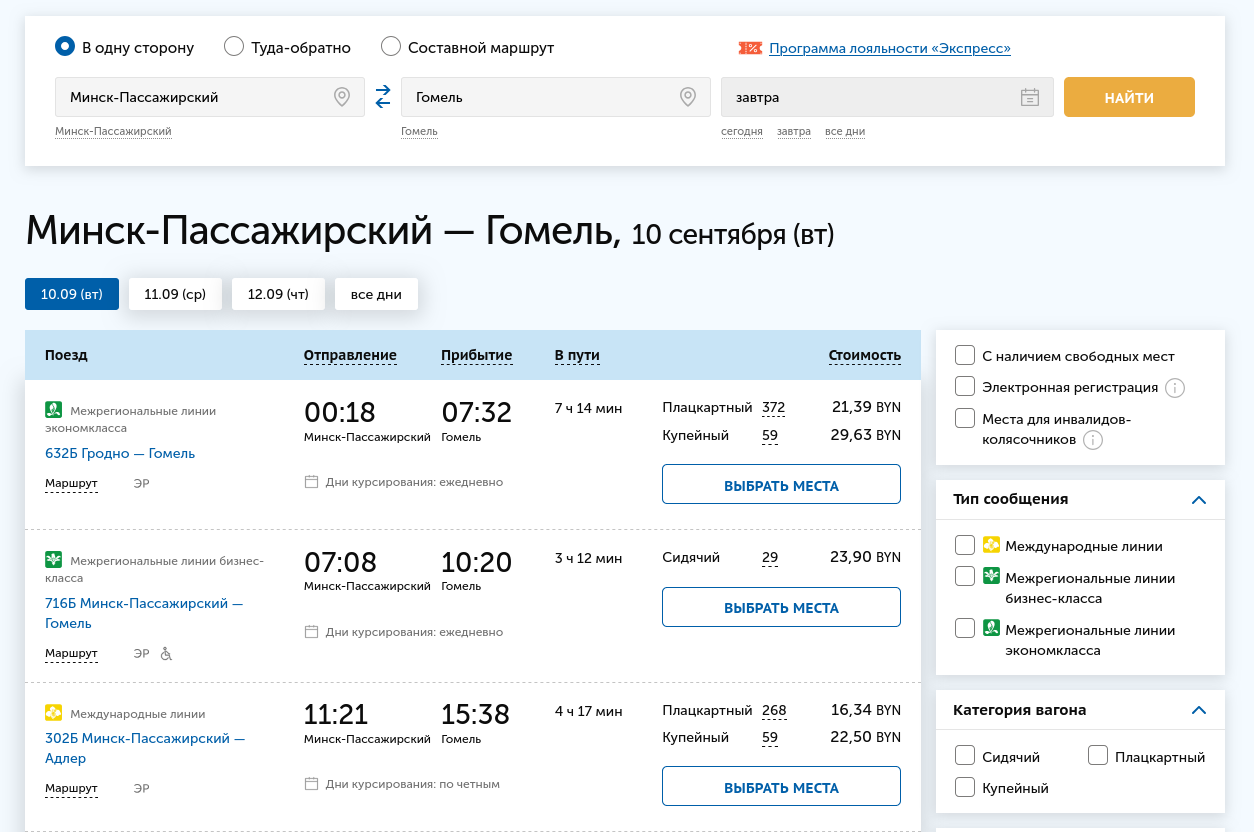
\includegraphics[width=0.8\textwidth]{1.2.png}
    \caption{Страница выбранного направления}
  \end{figure}

После ввода данных о поездке, сервис предлагает выбрать поезд. Так же указано количество мест и цена. Чтобы выбрать места необходимо нажать на кнопку <<Выбрать места>> для необходимого поезда. (Рисунок 1.3)  \\

\begin{figure}[h]
  \centering
  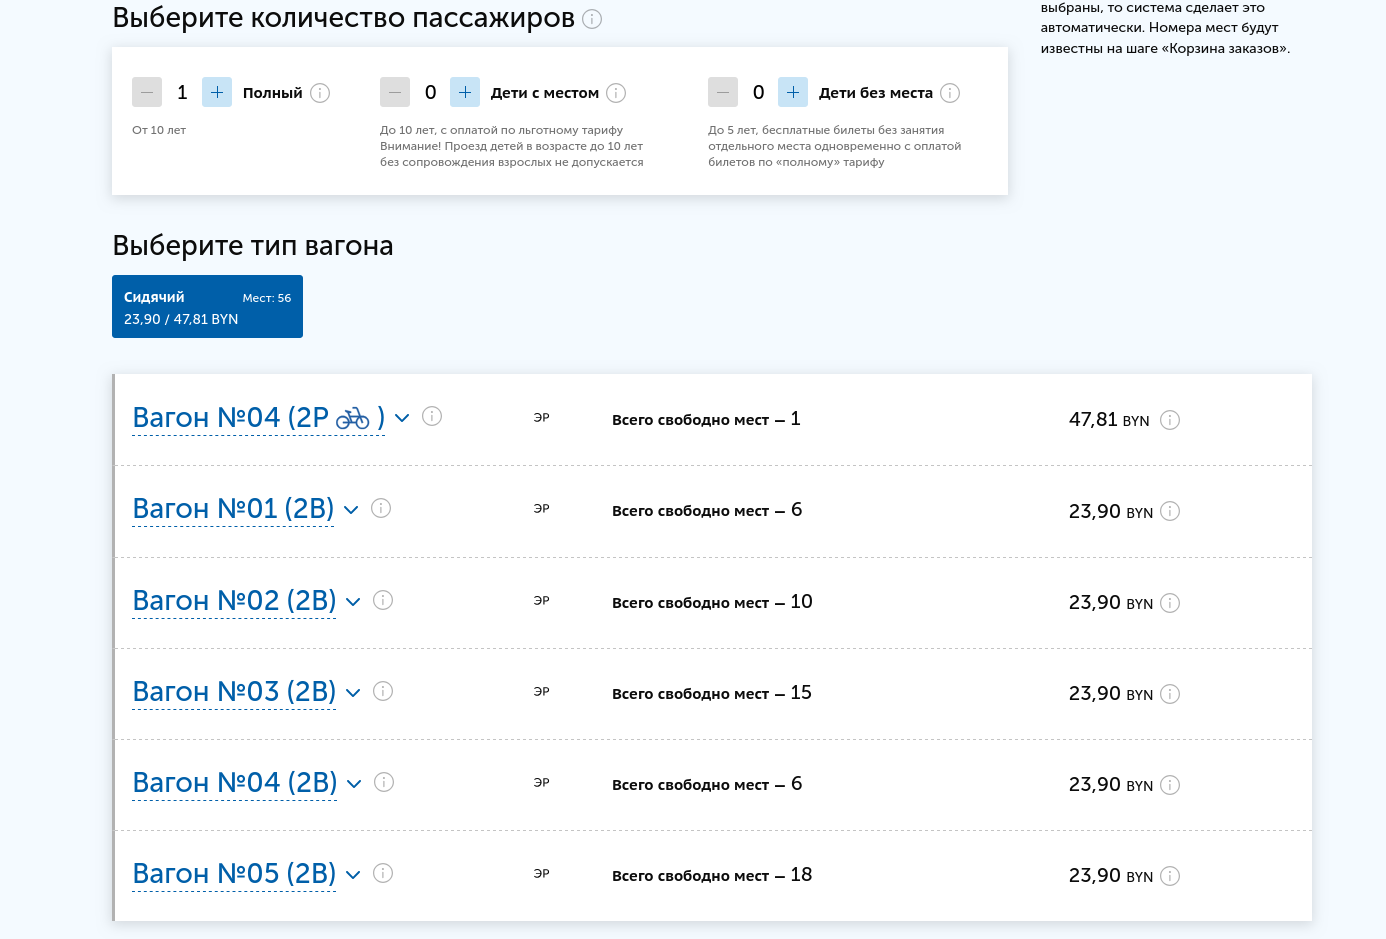
\includegraphics[width=0.75\textwidth]{1.3.png}
  \caption{Страница выбора вагона}
\end{figure}

После нажатия на кнопку <<Выбрать места>> необходимо выбрать вагон, в результате чего откроется окно выбора мест, где свободные места имеют белый фон, а занятые -- серый. Также, можно не выбирать конкретное место. В таком случае оно будет предложено системой. (Рисунок 1.4) \\

\begin{figure}[h]
  \centering
  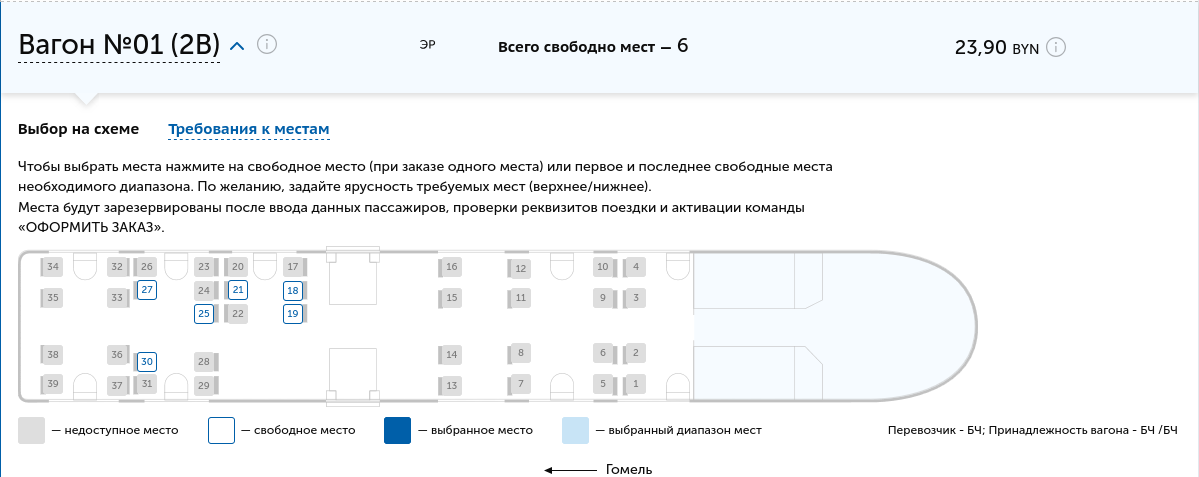
\includegraphics[width=0.75\textwidth]{1.4.png}
  \caption{Страница выбора места}
\end{figure}

После выбора места, необходимо ввести данные о пассажире. Также, предусмотрена система выбора двух и более пассажиров. Билеты в таком случае можно оформить либо на одного, либо на двух и более людей. (Рисунок 1.5)\\

\begin{figure}[h]
  \centering
  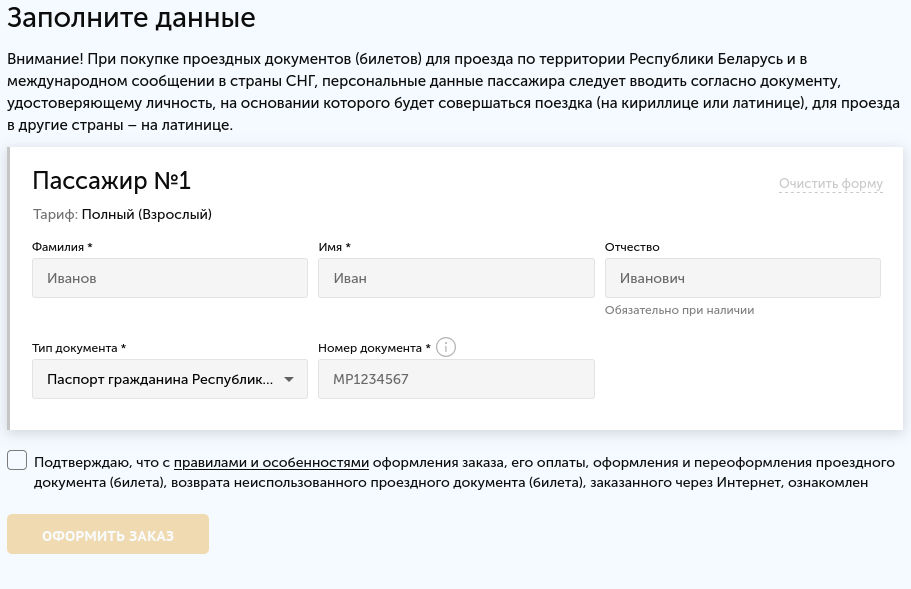
\includegraphics[width=1\textwidth]{1.5.png}
  \caption{Страница ввода данных о пассажире}
\end{figure}

После ввода данных о пассажире, заказ будет создан и помещен в корзину, которую необходимо оплатить в течении 20 минут. Эти 20 минут, билет будет зарезервирован и никто другой не сможет его взять.
\subsection{Постановка задачи на курсовое проектирование}

В данной курсовой работе необходимо разработать структуру иерархии классов информационной системы транспортной компании. Также необходимо отразить с помощью диаграмм структуру классов и их иерархии и с помощью блок-схемы отобразить ход работы алгоритма.
Для реализации поставленных задач необходимо следующее:
\begin{itemize}
  \item разработать иерархию классов, определить базовый и наследуемые классы;
  \item разработать и описать структуру каждого класса в отдельности, объявить поля и методы класса;
  \item реализовать программу для работы с иерархией классов.
\end{itemize}
Так как основным способом реализации консольного приложения в данной работе является объектно-ориентированное программирование на языке \textit{C++}, то структура приложения предполагает наличие базового и производных классов, то есть их иерархию, а также наличие полей и методов, которые описывают класс и позволяют взаимодействовать между объектами, воздействовать на сам объект и выполнять объекту определённые функции.

По требованию пользователя должно быть выполнено следующее действие:

\begin{itemize}
\item выбор маршрута рейса;
\item выбор даты и времени рейса;
\item изменение штата работников;
\item демонстрация возможностей системы;
\item возможность возвращения на предыдущий этап взаимодействия;
\item безопасное завершение работы программы.
\end{itemize}
